\documentclass[border=10pt]{standalone}
%%%<
\usepackage{verbatim}
%%%>
\usepackage{pgfplots}
\pgfplotsset{width=7cm,compat=1.8}
\usepackage{pgfplotstable}
\begin{comment}
:Title: Bar chart with multiple series
:Tags: 2D;Bar charts;Economy
:Author: Jake
:Slug: multi-series-bar-chart

Similar to the "Economist" style, we don't use a vertical grid,
avoid tick marks, and place the axis at the right, to highlight
the latest data.

This code was written by Jake on TeX.SE.
\end{comment}
\renewcommand*{\familydefault}{\sfdefault}
\usepackage{sfmath}
\begin{document}
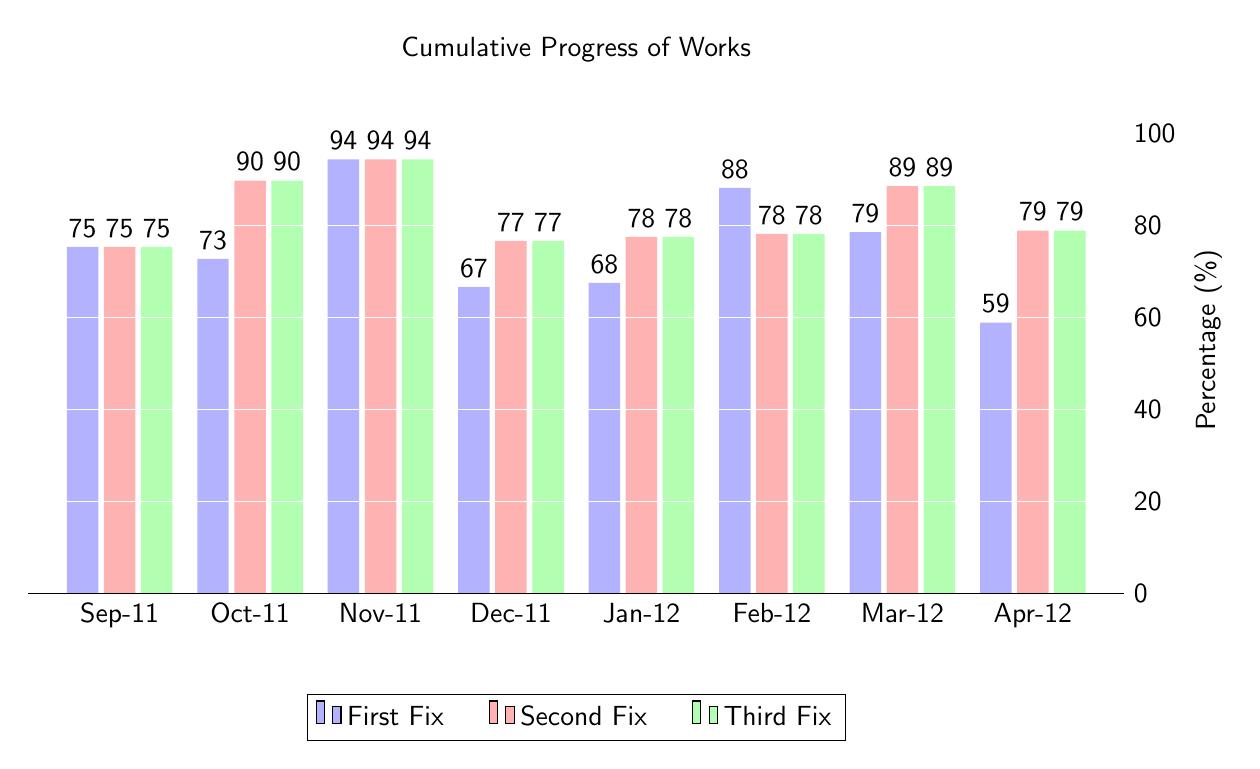
\begin{tikzpicture}
  \centering
  \begin{axis}[
        ybar, axis on top,
        title={Cumulative Progress of Works},
        height=8cm, width=15.5cm,
        bar width=0.4cm,
        ymajorgrids, tick align=inside,
        major grid style={draw=white},
        enlarge y limits={value=.1,upper},
        ymin=0, ymax=100,
        axis x line*=bottom,
        axis y line*=right,
        y axis line style={opacity=0},
        tickwidth=0pt,
        enlarge x limits=true,
        legend style={
            at={(0.5,-0.2)},
            anchor=north,
            legend columns=-1,
            /tikz/every even column/.append style={column sep=0.5cm}
        },
        ylabel={Percentage (\%)},
        symbolic x coords={
           Sep-11,Oct-11,Nov-11,Dec-11,
           Jan-12,Feb-12,
           Mar-12,
          Apr-12},
       xtick=data,
       nodes near coords={
        \pgfmathprintnumber[precision=0]{\pgfplotspointmeta}
       }
    ]
    \addplot [draw=none, fill=blue!30] coordinates {
      (Sep-11,75.4064)
      (Oct-11, 72.7961) 
      (Nov-11,94.4597)
      (Dec-11,66.6786) 
      (Jan-12,67.5600) 
      (Feb-12,88.2339)
      (Mar-12,78.6138) 
      (Apr-12,58.9129) };
   \addplot [draw=none,fill=red!30] coordinates {
      (Sep-11,75.4064)
      (Oct-11, 89.7961) 
      (Nov-11,94.4597)
      (Dec-11,76.6786) 
      (Jan-12,77.5600) 
      (Feb-12,78.2339)
      (Mar-12,88.6138) 
      (Apr-12,78.9129) };
   \addplot [draw=none, fill=green!30] coordinates {
      (Sep-11,75.4064)
      (Oct-11, 89.7961) 
      (Nov-11,94.4597)
      (Dec-11,76.6786) 
      (Jan-12,77.5600) 
      (Feb-12,78.2339)
      (Mar-12,88.6138) 
      (Apr-12,78.9129) };

    \legend{First Fix,Second Fix,Third Fix}
  \end{axis}
  \end{tikzpicture}
\end{document}
